% !TEX program = tectonic
% ============================================================================
% FROM ONE SIMULATION TO A TOOLKIT
% How the Pallet Handling Simulation (revC, PR99) is built, and how to
% platformize it into a reusable digital-twin toolkit.
% ============================================================================
\documentclass[11pt,a4paper]{article}

\usepackage[utf8]{inputenc}
\usepackage[T1]{fontenc}
\usepackage{lmodern}
\usepackage[margin=2.2cm]{geometry}
\usepackage{amsmath,amssymb}
\usepackage{graphicx}
\usepackage{xcolor}
\usepackage{tikz}
\usetikzlibrary{arrows.meta,positioning,shapes.geometric,fit,calc,backgrounds,decorations.pathreplacing}
\usepackage{booktabs}
\usepackage{array}
\usepackage{tabularx}
\usepackage{enumitem}
\usepackage{listings}
\usepackage[hidelinks]{hyperref}
\usepackage{fancyhdr}
\usepackage{titlesec}
\usepackage{parskip}
\usepackage{caption}
\usepackage{float}
\raggedbottom
\sloppy

\definecolor{inkP}{HTML}{0F172A}
\definecolor{inkM}{HTML}{64748B}
\definecolor{pxblue}{RGB}{21,67,116}
\definecolor{pxteal}{RGB}{0,128,128}
\definecolor{pxorange}{RGB}{204,102,0}
\definecolor{pxgray}{RGB}{245,246,248}
\definecolor{pxgreen}{RGB}{34,111,60}
\definecolor{pxred}{RGB}{165,42,42}

\titleformat{\section}{\Large\bfseries\color{pxblue}}{\thesection}{0.6em}{}
\titleformat{\subsection}{\large\bfseries\color{inkP}}{\thesubsection}{0.6em}{}
\pagestyle{fancy}
\fancyhf{}
\fancyhead[L]{\small\color{inkM}Pallet Handling Simulation $\rightarrow$ Toolkit}
\fancyhead[R]{\small\color{inkM}ParaTech Platform R\&D}
\fancyfoot[C]{\small\thepage}
\renewcommand{\headrulewidth}{0.3pt}

\lstset{basicstyle=\ttfamily\footnotesize, breaklines=true, frame=single,
  rulecolor=\color{pxblue!40}, backgroundcolor=\color{pxgray},
  columns=fullflexible, keepspaces=true, showstringspaces=false}

\tikzset{
  box/.style={draw=pxblue, thick, rounded corners=2pt, fill=pxgray,
    align=center, font=\footnotesize, inner sep=4pt, minimum height=8mm},
  sys/.style={draw=pxblue, thick, rounded corners=2pt, fill=pxblue!10,
    align=center, font=\footnotesize\bfseries, inner sep=4pt, minimum height=9mm},
  newb/.style={draw=pxorange, thick, rounded corners=2pt, fill=pxorange!10,
    align=center, font=\footnotesize\bfseries, inner sep=4pt, minimum height=9mm},
  ext/.style={draw=pxteal, thick, rounded corners=2pt, fill=pxteal!10,
    align=center, font=\footnotesize, inner sep=4pt, minimum height=8mm},
  data/.style={draw=pxgreen, thick, fill=pxgreen!10, align=center,
    font=\footnotesize, inner sep=4pt, minimum height=8mm,
    shape=rectangle, rounded corners=6pt},
  flow/.style={-{Stealth[length=2.2mm]}, thick, pxblue},
  flow2/.style={-{Stealth[length=2.2mm]}, thick, pxteal, dashed},
  flow3/.style={-{Stealth[length=2.2mm]}, thick, pxorange},
  lbl/.style={font=\scriptsize, fill=white, inner sep=1pt},
  grp/.style={draw=pxblue!35, fill=pxblue!3, rounded corners=4pt, inner sep=7pt},
  grpo/.style={draw=pxorange!45, fill=pxorange!4, rounded corners=4pt, inner sep=7pt},
  gtitle/.style={font=\scriptsize\bfseries, text=pxblue, anchor=south west, inner sep=2pt},
  gtitleo/.style={font=\scriptsize\bfseries, text=pxorange, anchor=south west, inner sep=2pt},
}

\begin{document}

\begin{titlepage}
\centering\vspace*{3cm}
{\color{pxblue}\rule{\linewidth}{1.2pt}}\\[6mm]
{\Huge\bfseries From One Simulation to a Toolkit\par}
\vspace{4mm}
{\Large How the \emph{Pallet Handling Simulation} (revC, PR99) is built,\\and how to platformize it into a reusable digital-twin toolkit\par}
\vspace{4mm}
{\color{pxblue}\rule{\linewidth}{1.2pt}}\\[2cm]
{\large ParaTech Platform R\&D Team, ParagonCorp\par}
\vspace{2mm}
{\normalsize Technical note, October 2026\par}
\vspace{2cm}
\begin{minipage}{0.85\linewidth}
\small\textbf{Scope.} This note reverse-engineers the single-file artefact
\texttt{Pallet\_Handling\_Simulation\_revC\_PR99\_5365.html} (28.8\,MB) --
its asset pipeline, runtime stack, discrete-event engine and authoring
contracts -- and proposes a toolkit architecture, scenario manifest and
phased plan that turns this one-off build into a repeatable product for
other packing lines, distribution-centre cells and vendor equipment.
\end{minipage}
\vfill
\end{titlepage}

\tableofcontents
\newpage

% ============================================================================
\section{Executive Summary}
% ============================================================================
The Pallet Handling Simulation is a real-time 3D digital twin of a pallet-handling
cell: AMRs, a pallet changer, two Helix~3~Evo stretch wrappers, a PR99 four-way strapper,
forklifts and truck bays. It compares two layout options (compact vs.\ buffered) and reports
throughput, lead time and utilisation so that a layout and forklift count can be chosen.
It ships as \emph{one self-contained HTML file}: two compressed glTF models, two textures and a
bundled JavaScript application (three.js plus the simulation, roughly 27\,KB of minified app code).

\textbf{Key observations.}
\begin{itemize}[leftmargin=*,itemsep=2pt]
  \item The build is \emph{craft-made but well structured}: a Blender-authored model whose node names
        and \texttt{extras} tags form an implicit API, driven by a fixed-timestep (0.05\,s) discrete-event
        engine built from four primitives (tween, lane/slot, load, agent).
  \item About 97\,\% of the file is model payload (${\sim}$492\,k triangles per option). Code and
        scenario knowledge (lane tables, waypoints, parameters) are \emph{hard-coded} in the minified bundle.
  \item Reuse today means copying the file and editing minified code. That does not scale.
\end{itemize}

\textbf{Recommendation.} Extract the engine into a scenario-agnostic \emph{core}, move every piece of
scenario knowledge into a validated \emph{scenario manifest} (JSON) that is bound to a named-node
\emph{asset contract}, add a headless \emph{batch runner} for multi-replication KPI studies, and wrap
all of it in an authoring CLI and a viewer shell. Section~\ref{sec:toolkit} specifies the target;
Section~\ref{sec:roadmap} phases the work; the first milestone reproduces revC bit-for-bit
from a manifest.

% ============================================================================
\section{How the Simulation Is Built}
\label{sec:build}
% ============================================================================

\subsection{Build pipeline: from CAD to a single HTML file}

Figure~\ref{fig:pipeline} shows the end-to-end path. Equipment is modelled in Blender (vendor CAD
imported or re-modelled), tagged with names and \texttt{extras.grp}, exported as glTF\,2.0
(Khronos I/O 4.3, Y-up, metres), gzip-compressed, base64-encoded and inlined into
\texttt{<script type="application/octet-stream">} blocks. The JavaScript bundle and two small
PNG textures are inlined beside them.

\begin{figure}[htbp]
\centering
\resizebox{\linewidth}{!}{%
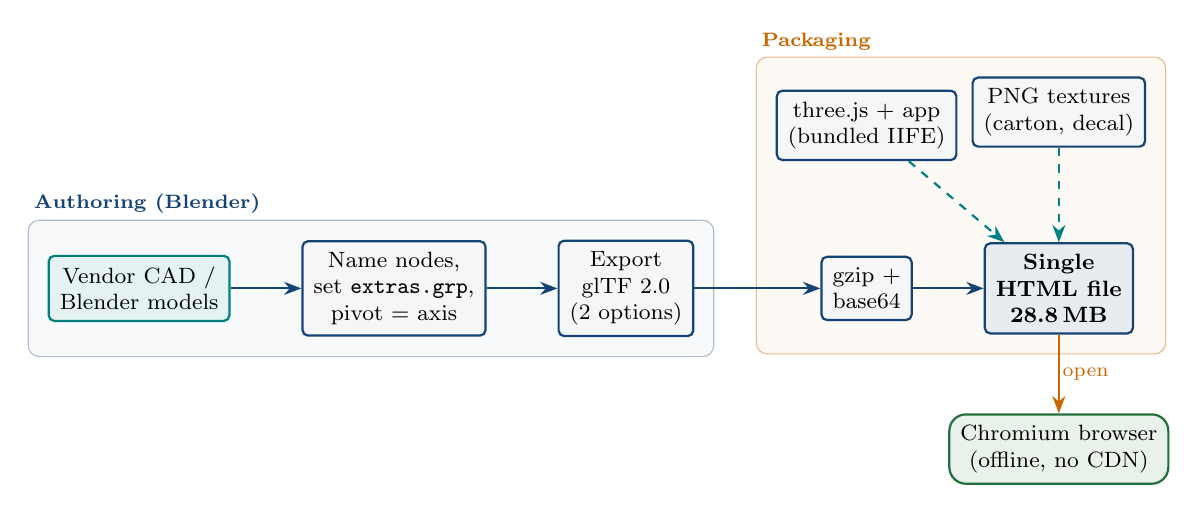
\begin{tikzpicture}[node distance=7mm and 9mm]
  \node[ext] (cad) {Vendor CAD /\\Blender models};
  \node[box, right=of cad] (tag) {Name nodes,\\set \texttt{extras.grp},\\pivot = axis};
  \node[box, right=of tag] (glb) {Export\\glTF 2.0\\(2 options)};
  \node[box, right=16mm of glb] (gz) {gzip +\\base64};
  \node[sys, right=of gz] (html) {Single\\HTML file\\28.8\,MB};
  \node[box, above=12mm of gz] (code) {three.js + app\\(bundled IIFE)};
  \node[box, above=12mm of html] (tex) {PNG textures\\(carton, decal)};
  \draw[flow] (cad)--(tag); \draw[flow] (tag)--(glb); \draw[flow] (glb)--(gz); \draw[flow] (gz)--(html);
  \draw[flow2] (code)--(html); \draw[flow2] (tex)--(html);
  \node[data, below=10mm of html] (br) {Chromium browser\\(offline, no CDN)};
  \draw[flow3] (html)--node[lbl,right]{open}(br);
  \begin{scope}[on background layer]
    \node[grp, fit=(cad)(tag)(glb)] (g1) {};
    \node[grpo, fit=(gz)(html)(code)(tex)] (g2) {};
    \node[gtitle] at (g1.north west) {Authoring (Blender)};
    \node[gtitleo] at (g2.north west) {Packaging};
  \end{scope}
\end{tikzpicture}}
\caption{Build pipeline of revC. Solid arrows: model payload; dashed: code and textures inlined at packaging.}
\label{fig:pipeline}
\end{figure}

\begin{table}[htbp]
\centering\small
\begin{tabularx}{\linewidth}{@{}l l X@{}}
\toprule
\textbf{Region (lines)} & \textbf{Size} & \textbf{Content}\\
\midrule
1--68 & small & HTML head and CSS (dark theme, fixed panes)\\
69--98 & ${\sim}$41\,KB & DOM: canvas, control panel, KPI pane, loader, tag overlay, inline logos\\
100 / 101 & ${\sim}$14\,MB each & \texttt{glb1}, \texttt{glb2}: Option~1 / Option~2 models (gzip + base64)\\
102 & ${\sim}$99\,KB & \texttt{window.TEX}: carton and trailer-decal PNG data URIs\\
103--end & ${\sim}$0.4\,MB & Bundled IIFE: three.js (GLTFLoader, OrbitControls, PMREM) + simulation\\
\bottomrule
\end{tabularx}
\caption{Anatomy of the 28.8\,MB file.}
\end{table}

\subsection{Runtime architecture}

At load time, the browser decodes \texttt{atob} $\rightarrow$ \texttt{DecompressionStream("gzip")}
$\rightarrow$ \texttt{GLTFLoader.parse}. Only Option~1 is parsed on start; Option~2 is parsed lazily on first
selection. Figure~\ref{fig:runtime} separates the four runtime layers and the single coupling point
between them: the \emph{named-node lookup}.

\begin{figure}[htbp]
\centering
\resizebox{\linewidth}{!}{%
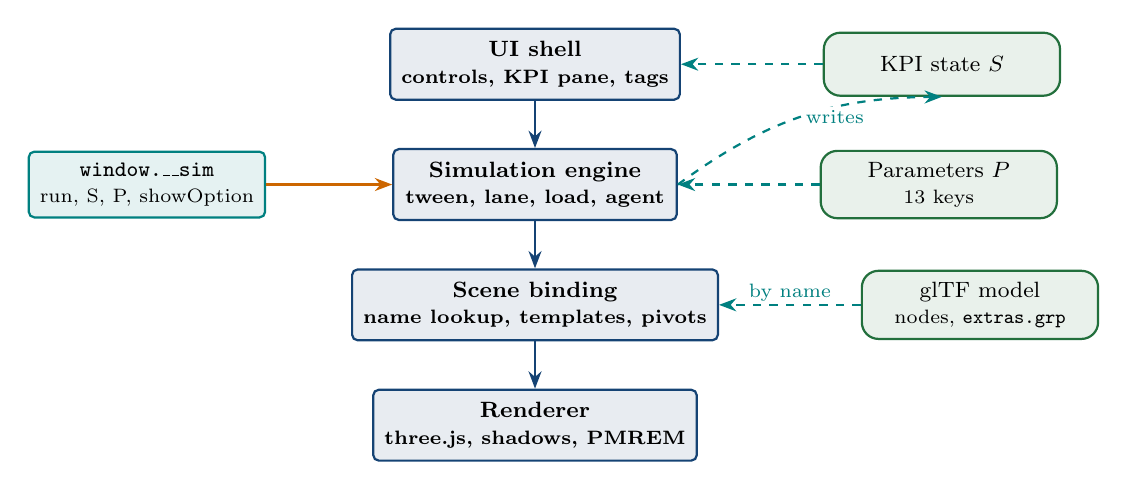
\begin{tikzpicture}[node distance=6mm]
  % layers
  \node[sys, minimum width=3.6cm] (ui) {UI shell\\\scriptsize controls, KPI pane, tags};
  \node[sys, minimum width=3.6cm, below=of ui] (sim) {Simulation engine\\\scriptsize tween, lane, load, agent};
  \node[sys, minimum width=3.6cm, below=of sim] (scene) {Scene binding\\\scriptsize name lookup, templates, pivots};
  \node[sys, minimum width=3.6cm, below=of scene] (r3d) {Renderer\\\scriptsize three.js, shadows, PMREM};
  \node[data, right=18mm of scene, minimum width=3cm] (glb) {glTF model\\\scriptsize nodes, \texttt{extras.grp}};
  \node[data, right=18mm of sim, minimum width=3cm] (par) {Parameters $P$\\\scriptsize 13 keys};
  \node[data, right=18mm of ui, minimum width=3cm] (kpi) {KPI state $S$};
  \draw[flow] (ui) -- (sim);
  \draw[flow] (sim) -- (scene);
  \draw[flow] (scene) -- (r3d);
  \draw[flow2] (glb) -- node[lbl,above]{by name}(scene);
  \draw[flow2] (par) -- (sim);
  \draw[flow2] (sim.east) to[bend left=18] node[lbl,right]{writes}(kpi.south);
  \draw[flow2] (kpi) -- (ui);
  \node[ext, left=16mm of sim, minimum width=2.4cm] (hook) {\texttt{window.\_\_sim}\\\scriptsize run, S, P, showOption};
  \draw[flow3] (hook) -- (sim);
\end{tikzpicture}}
\caption{Runtime layers. The headless hook \texttt{window.\_\_sim} is the seed of the batch runner.}
\label{fig:runtime}
\end{figure}

\textbf{Rendering.} perspective camera (FOV~40$^\circ$), ACES-style tone mapping (exposure 0.85), one warm
directional light with a $4096^2$ shadow map, a weak hemisphere fill, and a \emph{procedural}
image-based environment (a small room of emissive boxes through PMREM) -- no HDRI file.
Sim space is 2-D $(x,y)$ on the floor, mapped to three.js as $(x,\,h,\,-y)$, in metres.

\subsection{The 3D asset contract}

Each option is a glTF of ${\sim}$24.7\,MB uncompressed: ${\sim}$492\,k triangles, 569--600 nodes, ${\sim}$350 meshes,
${\sim}$137 materials, \emph{zero animations and zero skins}. All motion is code-driven.
The code and the model are bound by five conventions (Figure~\ref{fig:contract}):

\begin{enumerate}[leftmargin=*,itemsep=2pt]
  \item \textbf{Name-based lookup} (e.g.\ \texttt{RotatingArm\_PIVOT}, \texttt{FilmCarriage\_Z},
        \texttt{PR99\_Sword}, \texttt{Forklift\_Outside\_Truck}). A rename breaks the sim silently.
  \item \textbf{Layer tags} via \texttt{extras.grp}: \texttt{pc, line1, line2, fence, loads, walls, forklifts, buffer, trucks, floor}.
  \item \textbf{Pivot = animation axis.} Origin at the pivot; the rest pose is stored on load and animation is relative to it.
  \item \textbf{Hidden templates, cloned at runtime} (loads, AMR, forklift) and re-based to bottom-centre.
  \item \textbf{Materials keyed by name} and re-skinned in code (wood, film, floor, carton logo, decal).
\end{enumerate}

\begin{figure}[htbp]
\centering
\resizebox{\linewidth}{!}{%
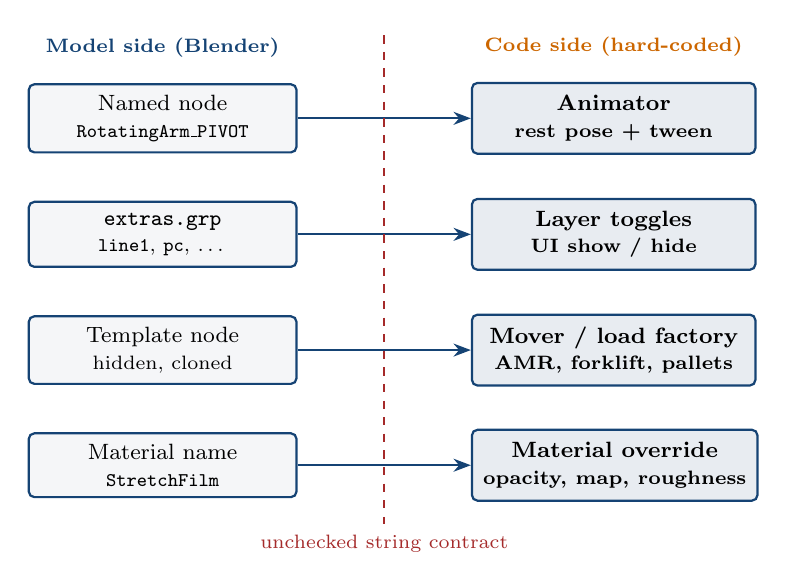
\begin{tikzpicture}[node distance=6mm and 10mm]
  \node[box, minimum width=3.4cm] (n1) {Named node\\\scriptsize \texttt{RotatingArm\_PIVOT}};
  \node[box, minimum width=3.4cm, below=of n1] (n2) {\texttt{extras.grp}\\\scriptsize \texttt{line1}, \texttt{pc}, \dots};
  \node[box, minimum width=3.4cm, below=of n2] (n3) {Template node\\\scriptsize hidden, cloned};
  \node[box, minimum width=3.4cm, below=of n3] (n4) {Material name\\\scriptsize \texttt{StretchFilm}};
  \node[sys, right=22mm of n1, minimum width=3.6cm] (b1) {Animator\\\scriptsize rest pose + tween};
  \node[sys, right=22mm of n2, minimum width=3.6cm] (b2) {Layer toggles\\\scriptsize UI show / hide};
  \node[sys, right=22mm of n3, minimum width=3.6cm] (b3) {Mover / load factory\\\scriptsize AMR, forklift, pallets};
  \node[sys, right=22mm of n4, minimum width=3.6cm] (b4) {Material override\\\scriptsize opacity, map, roughness};
  \foreach \i in {1,2,3,4}{\draw[flow] (n\i)--(b\i);}
  \node[font=\scriptsize\bfseries, above=2mm of n1, text=pxblue] {Model side (Blender)};
  \node[font=\scriptsize\bfseries, above=2mm of b1, text=pxorange] {Code side (hard-coded)};
  \draw[pxred, thick, dashed, rounded corners] ($(n1.north east)!0.5!(b1.north west)+(0,0.6)$) -- ($(n4.south east)!0.5!(b4.south west)+(0,-0.3)$);
  \node[font=\scriptsize, text=pxred, fill=white, inner sep=1pt] at ($(n4.east)!0.5!(b4.west)+(0,-1.0)$) {unchecked string contract};
\end{tikzpicture}}
\caption{The implicit model--code contract. Every arrow is a string match that nothing validates.}
\label{fig:contract}
\end{figure}

\subsection{Process model of the cell}

The simulated cell moves one product from production to a truck. Figure~\ref{fig:process} shows
the flow including the routing decision (tall loads to Line~1 with strapping, short loads to Line~2).

\begin{figure}[htbp]
\centering
\resizebox{\linewidth}{!}{%
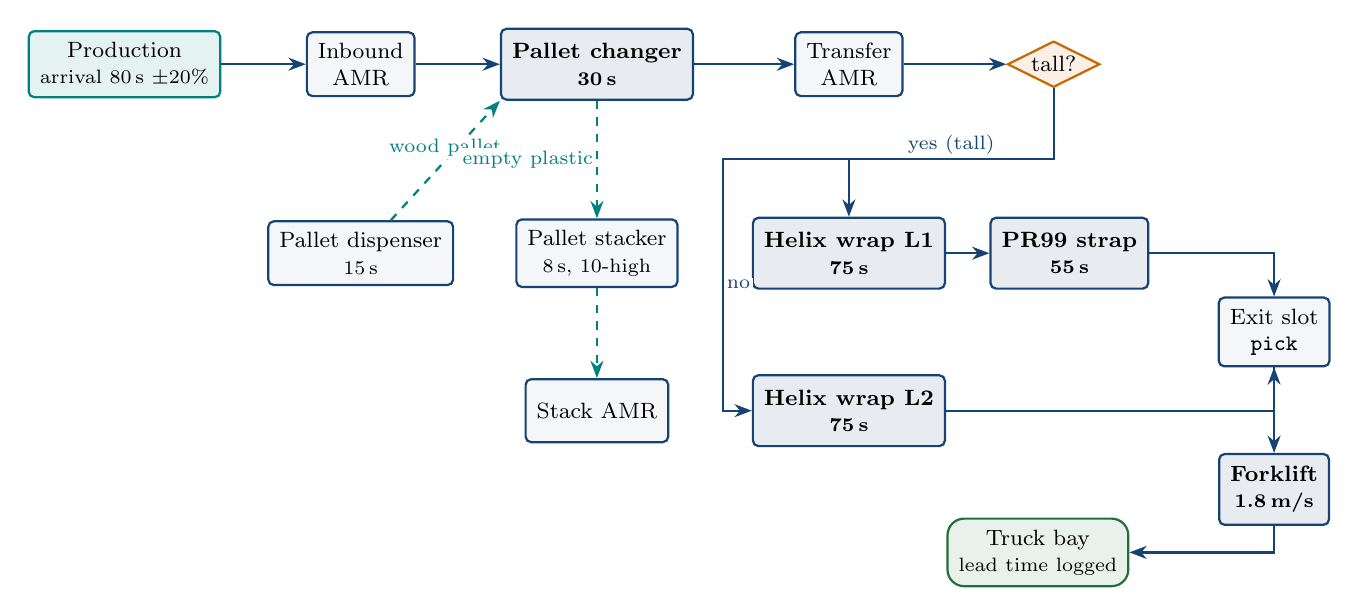
\begin{tikzpicture}
  \node[ext]  (prod) at (0,0)   {Production\\\scriptsize arrival 80\,s $\pm$20\%};
  \node[box]  (amr1) at (3,0)   {Inbound\\AMR};
  \node[sys]  (pc)   at (6,0)   {Pallet changer\\\scriptsize 30\,s};
  \node[box]  (amr2) at (9.2,0) {Transfer\\AMR};
  \node[diamond, draw=pxorange, thick, fill=pxorange!10, aspect=2, font=\footnotesize, inner sep=1pt] (dec) at (11.8,0) {tall?};
  \node[sys]  (w1) at (9.2,-2.4)  {Helix wrap L1\\\scriptsize 75\,s};
  \node[sys]  (st) at (12,-2.4)   {PR99 strap\\\scriptsize 55\,s};
  \node[sys]  (w2) at (9.2,-4.4)  {Helix wrap L2\\\scriptsize 75\,s};
  \node[box]  (pick) at (14.6,-3.4) {Exit slot\\\texttt{pick}};
  \node[sys]  (fk)   at (14.6,-5.4) {Forklift\\\scriptsize 1.8\,m/s};
  \node[data] (truck) at (11.6,-6.2) {Truck bay\\\scriptsize lead time logged};
  \node[box]  (disp) at (3,-2.4)  {Pallet dispenser\\\scriptsize 15\,s};
  \node[box]  (stack) at (6,-2.4) {Pallet stacker\\\scriptsize 8\,s, 10-high};
  \node[box]  (amr3) at (6,-4.4)  {Stack AMR};
  \draw[flow] (prod)--(amr1); \draw[flow] (amr1)--(pc); \draw[flow] (pc)--(amr2); \draw[flow] (amr2)--(dec);
  \draw[flow] (dec.south) -- (11.8,-1.2) -- node[lbl,pos=0.5,above]{yes (tall)} (9.2,-1.2) -- (w1.north);
  \draw[flow] (11.8,-1.2) -- (7.6,-1.2) -- node[lbl,pos=0.5,right]{no} (7.6,-4.4) -- (w2.west);
  \draw[flow] (w1)--(st); \draw[flow] (st) -| (pick); \draw[flow] (w2) -| (pick);
  \draw[flow] (pick)--(fk); \draw[flow] (fk)|-(truck);
  \draw[flow2] (disp)--node[lbl,above]{wood pallet}(pc.south west);
  \draw[flow2] (pc)--node[lbl,left]{empty plastic}(stack);
  \draw[flow2] (stack)--(amr3);
\end{tikzpicture}}
\caption{Material flow of revC. Solid: loaded product; dashed: empty pallets. Times are default concept assumptions.}
\label{fig:process}
\end{figure}

\subsection{Simulation engine}

The engine is a \emph{fixed-timestep discrete-event/time-stepped hybrid}: simulated time advances in
$\Delta t = 0.05$\,s steps; the render loop accumulates $\text{realDelta}\times\text{speed}$ (real delta clamped to
0.1\,s, at most 2000 steps per frame) and steps the engine as many times as needed. Randomness is a
single Lehmer LCG (seed 7, multiplier 16807 mod $2^{31}-1$), reset on every Restart, which makes Option~1 vs.\ Option~2
runs directly comparable.

\begin{figure}[htbp]
\centering
\resizebox{\linewidth}{!}{%
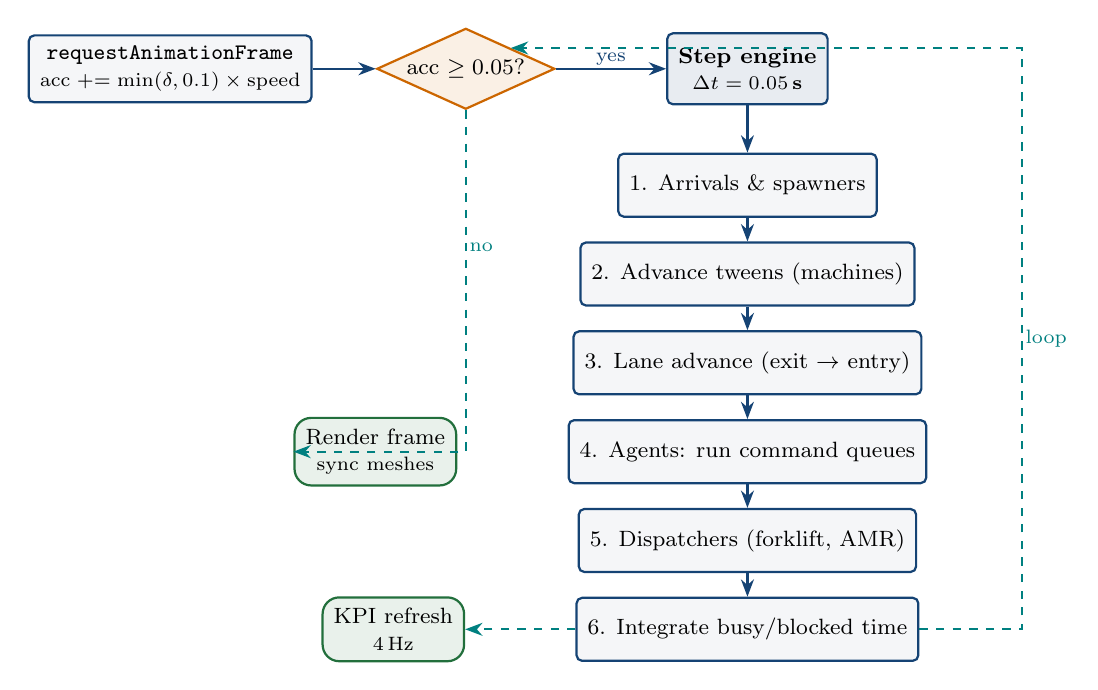
\begin{tikzpicture}[node distance=6mm and 8mm]
  \node[box] (raf) {\texttt{requestAnimationFrame}\\\scriptsize $\text{acc} \mathrel{+}= \min(\delta,0.1)\times\text{speed}$};
  \node[diamond, draw=pxorange, thick, fill=pxorange!10, aspect=2.2, font=\footnotesize, inner sep=1pt, right=of raf] (chk) {acc $\ge 0.05$?};
  \node[sys, right=14mm of chk] (step) {Step engine\\\scriptsize $\Delta t = 0.05$\,s};
  \node[box, below=of step] (a) {1. Arrivals \& spawners};
  \node[box, below=3mm of a] (b) {2. Advance tweens (machines)};
  \node[box, below=3mm of b] (c) {3. Lane advance (exit $\rightarrow$ entry)};
  \node[box, below=3mm of c] (d) {4. Agents: run command queues};
  \node[box, below=3mm of d] (e) {5. Dispatchers (forklift, AMR)};
  \node[box, below=3mm of e] (f) {6. Integrate busy/blocked time};
  \node[data, left=14mm of d] (render) {Render frame\\\scriptsize sync meshes};
  \node[data, left=14mm of f] (kpi) {KPI refresh\\\scriptsize 4\,Hz};
  \draw[flow] (raf)--(chk);
  \draw[flow] (chk)--node[lbl,above]{yes}(step);
  \draw[flow] (step)--(a); \draw[flow] (a)--(b); \draw[flow] (b)--(c); \draw[flow] (c)--(d); \draw[flow] (d)--(e); \draw[flow] (e)--(f);
  \draw[flow2] (chk.south) |- node[lbl,pos=0.2,right]{no}(render.west);
  \draw[flow2] (f.east) -- ++(1.3,0) |- node[lbl,near start,right]{loop}(chk.north east);
  \draw[flow2] (f)--(kpi);
\end{tikzpicture}}
\caption{One frame of the engine loop. The loop is deterministic given seed, parameters and layout.}
\label{fig:tick}
\end{figure}

Four primitives carry the whole model:

\begin{table}[htbp]
\centering\small
\begin{tabularx}{\linewidth}{@{}l X@{}}
\toprule
\textbf{Primitive} & \textbf{Semantics}\\
\midrule
Tween $(d, \text{update}, \text{done})$ & Timed machine animation; every machine cycle is a tween advanced by $\Delta t$.\\
Lane $(\text{name}, y, \text{slots})$ & Ordered slots $\{x, \text{proc}, \text{occ}, \text{res}\}$; \texttt{proc} (\texttt{wrap, strap, pick, amr, hold, disp, stack}) runs when a load arrives.\\
Load $\{\text{kind}, H, \text{tall}, \text{born}, \dots\}$ & \texttt{product, wood, plastic, stack}; \texttt{born} gives lead time.\\
Agent (AMR / forklift) & Command queue of \texttt{path}, \texttt{lift}, \texttt{wait}, \texttt{call}; turn-in-place at 1.6\,rad/s, then drive; carries one load.\\
\bottomrule
\end{tabularx}
\caption{Engine primitives.}
\end{table}

\textbf{Lane rule.} Scanning from exit backwards, a \texttt{ready} and not \texttt{moving} load advances when the next slot
is free and unreserved, taking $\text{distance}/v_{conv}$ seconds ($v_{conv}=0.25$\,m/s). Conflicts between movers are avoided \emph{only}
through slot reservation.

\textbf{KPIs.} Throughput per hour (after 15\,min; rolling 60\,min past 1\,h), average lead time over the last 200 loads,
station busy/blocked/idle fractions, queue at production, loads waiting for forklift, forklift utilisation $=\text{busy}/\text{simTime}$.

\subsection{Limits of the current build}
\begin{itemize}[leftmargin=*,itemsep=1pt]
  \item Scenario knowledge (lane slot tables, waypoint polylines, home positions, stations) is hard-coded in minified code.
  \item Fixed hand-written waypoints, no path-finding or collision avoidance; machine state is boolean.
  \item One RNG stream; no warm-up period or replications, so KPIs are single-sample.
  \item 492\,k triangles per option, 28\,MB single file; names-as-API breaks silently.
  \item Parameters are concept assumptions, not calibrated to measured cycle times.
\end{itemize}

% ============================================================================
\section{Platformizing into a Toolkit}
\label{sec:toolkit}
% ============================================================================

\subsection{Design principles}
\begin{enumerate}[leftmargin=*,itemsep=2pt]
  \item \textbf{Separate what changes from what does not.} Engine primitives are stable; layouts, lanes, cycle times and models change per scenario.
  \item \textbf{Data over code.} Every hard-coded table in revC becomes a field in a validated manifest.
  \item \textbf{One contract, checked at build time.} The names-as-API contract is declared once and verified against the glTF before any run.
  \item \textbf{Simulation is not rendering.} The engine runs headless in Node/Worker; the 3D viewer is an optional consumer of its state.
  \item \textbf{Reproducible by default.} Seeded streams, replications, versioned manifests and models.
\end{enumerate}

\subsection{Target architecture}

\begin{figure}[H]
\centering
\resizebox{\linewidth}{!}{%
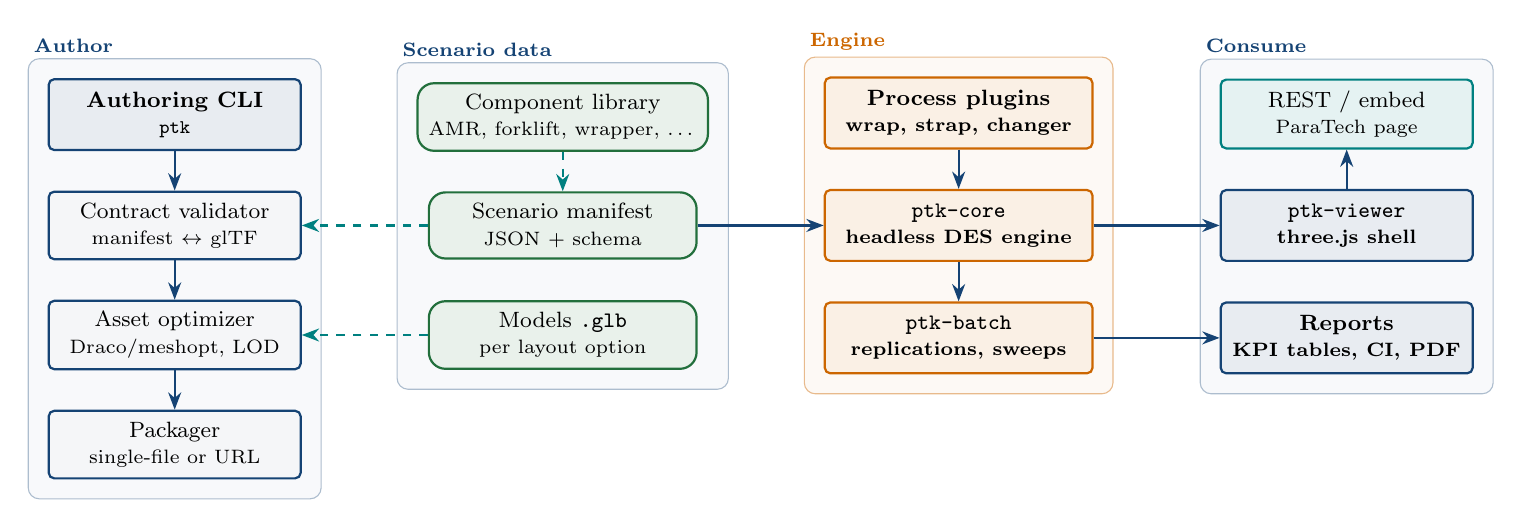
\begin{tikzpicture}[node distance=5mm and 7mm]
  % authoring
  \node[sys, minimum width=3.2cm] (cli) {Authoring CLI\\\scriptsize \texttt{ptk}};
  \node[box, below=of cli, minimum width=3.2cm] (val) {Contract validator\\\scriptsize manifest $\leftrightarrow$ glTF};
  \node[box, below=of val, minimum width=3.2cm] (opt) {Asset optimizer\\\scriptsize Draco/meshopt, LOD};
  \node[box, below=of opt, minimum width=3.2cm] (pack) {Packager\\\scriptsize single-file or URL};
  % data
  \node[data, right=16mm of val, minimum width=3.4cm] (man) {Scenario manifest\\\scriptsize JSON + schema};
  \node[data, right=16mm of opt, minimum width=3.4cm] (glb) {Models \texttt{.glb}\\\scriptsize per layout option};
  \node[data, above=of man, minimum width=3.4cm] (lib) {Component library\\\scriptsize AMR, forklift, wrapper, \dots};
  % core
  \node[newb, right=16mm of man, minimum width=3.4cm] (core) {\texttt{ptk-core}\\\scriptsize headless DES engine};
  \node[newb, below=of core, minimum width=3.4cm] (batch) {\texttt{ptk-batch}\\\scriptsize replications, sweeps};
  \node[newb, above=of core, minimum width=3.4cm] (plug) {Process plugins\\\scriptsize wrap, strap, changer};
  % outputs
  \node[sys, right=16mm of core, minimum width=3.2cm] (view) {\texttt{ptk-viewer}\\\scriptsize three.js shell};
  \node[sys, right=16mm of batch, minimum width=3.2cm] (rep) {Reports\\\scriptsize KPI tables, CI, PDF};
  \node[ext, above=of view, minimum width=3.2cm] (api) {REST / embed\\\scriptsize ParaTech page};
  \draw[flow] (cli)--(val); \draw[flow] (val)--(opt); \draw[flow] (opt)--(pack);
  \draw[flow2] (man)--(val); \draw[flow2] (glb)--(opt); \draw[flow2] (lib)--(man);
  \draw[flow] (man)--(core); \draw[flow] (plug)--(core); \draw[flow] (core)--(batch);
  \draw[flow] (core)--(view); \draw[flow] (batch)--(rep); \draw[flow] (view)--(api);
  \begin{scope}[on background layer]
    \node[grp, fit=(cli)(val)(opt)(pack)] (ga) {};
    \node[grp, fit=(man)(glb)(lib)] (gb) {};
    \node[grpo, fit=(core)(batch)(plug)] (gc) {};
    \node[grp, fit=(view)(rep)(api)] (gd) {};
    \node[gtitle] at (ga.north west) {Author};
    \node[gtitle] at (gb.north west) {Scenario data};
    \node[gtitleo] at (gc.north west) {Engine};
    \node[gtitle] at (gd.north west) {Consume};
  \end{scope}
\end{tikzpicture}}
\caption{Toolkit architecture. Orange blocks are new engineering; the viewer and engine are extracted from revC.}
\label{fig:arch}
\end{figure}

\subsection{Component responsibilities}

\begin{table}[H]
\centering\small
\begin{tabularx}{\linewidth}{@{}l X X@{}}
\toprule
\textbf{Component} & \textbf{Responsibility} & \textbf{Extracted from revC}\\
\midrule
\texttt{ptk-core} & Time loop, RNG streams, tween, lane, load, agent, KPI accumulators; no DOM, no three.js & Engine layer (\S\ref{sec:build})\\
Process plugins & Station behaviours (\texttt{wrap}, \texttt{strap}, \texttt{changer}, \texttt{stack}); register by \texttt{proc} name & Process logic table\\
\texttt{ptk-viewer} & Scene binding, animators, camera presets, tags, KPI panes & Renderer + UI layers\\
\texttt{ptk-batch} & Seeded replications, warm-up, parameter sweeps, confidence intervals & \texttt{\_\_sim.run}\\
Component library & Reusable machine/vehicle definitions: node names, pivots, travel, default cycle times & Asset catalogue\\
Validator & Fails the build if a manifest references a node, group or material the glTF lacks & (new)\\
Optimizer / packager & Draco/meshopt, decimation, split-asset or single-file export & Packaging step\\
\bottomrule
\end{tabularx}
\caption{Toolkit components and their origin.}
\end{table}

\subsection{The scenario manifest}

The manifest is the single source of scenario truth. It replaces the hard-coded lane tables, waypoints and
parameter object. The excerpt below encodes Line~1 of Option~1 and one parameter from revC.

\begin{lstlisting}[language=]
{
  "schema": "ptk.scenario/1",
  "model": { "glb": "options/compact.glb", "units": "m", "up": "Y" },
  "seed": 7,  "dt": 0.05,
  "lanes": [{
    "id": "L1", "y": -0.58,
    "slots": [
      { "x":  2.90 }, { "x":  1.00 },
      { "x": -1.595, "proc": "wrap",  "uses": "helix_L1" },
      { "x": -3.80 },
      { "x": -5.20,  "proc": "strap", "uses": "pr99" },
      { "x": -6.71,  "proc": "pick" }
    ]}],
  "stations": [{
    "id": "helix_L1", "plugin": "helix3evo", "cycle": {"param": "wrap"},
    "parts": { "arm": "RotatingArm_PIVOT", "carriage": "FilmCarriage_Z" }
  }],
  "agents": [{ "id": "fork1", "type": "forklift", "template": "Forklift_Outside_Truck",
               "speed": {"param": "fl"}, "home": [-10.6, -3.2] }],
  "params": { "wrap": { "label": "Wrapping cycle", "default": 75,
                        "min": 40, "max": 150, "step": 5, "unit": "s" } },
  "kpis": ["throughput_h", "lead_time_min", "util.station", "util.forklift"]
}
\end{lstlisting}

\subsection{Data flow with the manifest in the loop}

\begin{figure}[H]
\centering
\resizebox{\linewidth}{!}{%
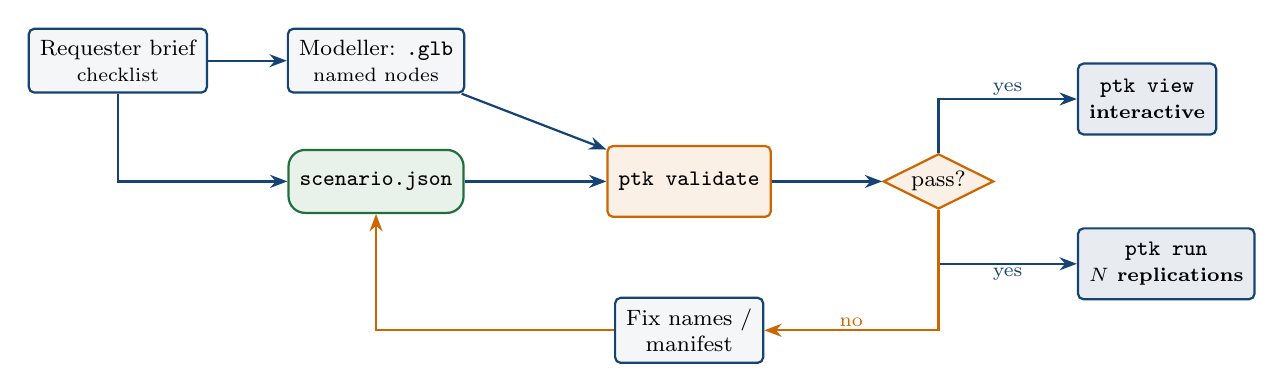
\begin{tikzpicture}[node distance=7mm and 10mm]
  \node[box] (brief) {Requester brief\\\scriptsize checklist};
  \node[box, right=of brief] (model) {Modeller: \texttt{.glb}\\\scriptsize named nodes};
  \node[data, below=of model] (man) {\texttt{scenario.json}};
  \node[newb, right=18mm of man] (val) {\texttt{ptk validate}};
  \node[diamond, draw=pxorange, thick, fill=pxorange!10, aspect=2, font=\footnotesize, inner sep=1pt, right=14mm of val] (ok) {pass?};
  \node[sys, above right=4mm and 14mm of ok] (view) {\texttt{ptk view}\\\scriptsize interactive};
  \node[sys, below right=4mm and 14mm of ok] (batch) {\texttt{ptk run}\\\scriptsize $N$ replications};
  \node[box, below=10mm of val] (fix) {Fix names /\\manifest};
  \draw[flow] (brief)--(model); \draw[flow] (brief)|-(man);
  \draw[flow] (model)--(val); \draw[flow] (man)--(val);
  \draw[flow] (val)--(ok);
  \draw[flow] (ok)|-node[lbl,near end,above]{yes}(view);
  \draw[flow] (ok)|-node[lbl,near end,below]{yes}(batch);
  \draw[flow3] (ok) |- node[lbl,near end,above]{no}(fix.east);
  \draw[flow3] (fix.west) -| (man.south);
\end{tikzpicture}}
\caption{Authoring loop. The validator turns silent name mismatches into build-time errors.}
\label{fig:loop}
\end{figure}

\subsection{From single sample to decision-grade statistics}

revC reports a single stochastic trajectory. For a layout decision the toolkit should report, per option and
parameter set, the mean and a confidence interval over $R$ independent replications after a warm-up of length $T_w$.
With replication means $\bar{X}_1,\dots,\bar{X}_R$ (e.g.\ throughput per hour),
\[
  \hat{\mu} = \frac{1}{R}\sum_{r=1}^{R}\bar{X}_r,\qquad
  \hat{\mu} \pm t_{R-1,\,1-\alpha/2}\,\frac{s}{\sqrt{R}} .
\]
Replications use independent seeded streams (split arrival, forklift-away and routing streams), and Option~A vs.\ Option~B are compared with
\emph{common random numbers} so that the paired difference isolates the layout effect. Because the engine is deterministic given
\texttt{(manifest, seed)}, every reported number is reproducible from a hash of those two inputs.

\subsection{Asset pipeline improvements}

\begin{table}[H]
\centering\small
\begin{tabularx}{\linewidth}{@{}l X X@{}}
\toprule
\textbf{Concern} & \textbf{revC} & \textbf{Toolkit}\\
\midrule
Model delivery & Base64 inline, 28\,MB & Separate \texttt{.glb} (Draco/meshopt), lazy per option; single-file export only for e-mail hand-off\\
Triangle budget & ${\sim}$492\,k per option & Target $<150$\,k, LOD for distant machines\\
Contract & Implicit string names & Component library declares names; validator enforces\\
Textures & Inline PNG data URIs & Separate files, KTX2 where useful\\
Hosting & Static file in an iframe, no file-level access control & Versioned assets behind the platform's auth\\
\bottomrule
\end{tabularx}
\caption{Asset pipeline: current vs.\ target.}
\end{table}

% ============================================================================
\section{Roadmap}
\label{sec:roadmap}
% ============================================================================

\begin{figure}[htbp]
\centering
\resizebox{\linewidth}{!}{%
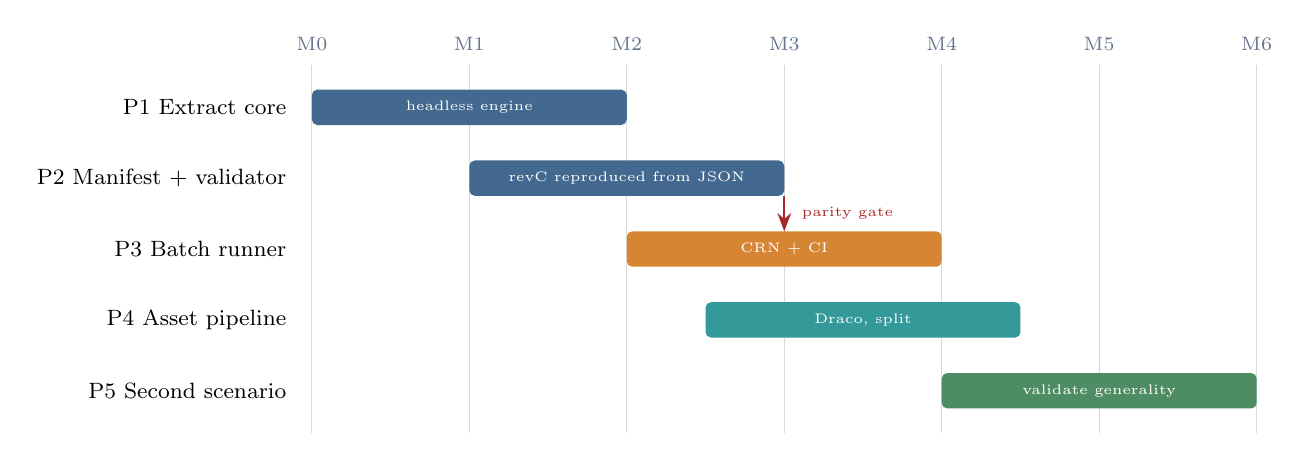
\begin{tikzpicture}[x=1.0cm, y=-0.9cm]
  \foreach \x/\t in {0/{M0},2/{M1},4/{M2},6/{M3},8/{M4},10/{M5},12/{M6}}{
    \node[font=\scriptsize, text=inkM] at (\x,-0.3) {\t};
    \draw[gray!30] (\x,0) -- (\x,5.2);}
  \node[anchor=east, font=\footnotesize] at (-0.2,0.6) {P1 Extract core};
  \node[anchor=east, font=\footnotesize] at (-0.2,1.6) {P2 Manifest + validator};
  \node[anchor=east, font=\footnotesize] at (-0.2,2.6) {P3 Batch runner};
  \node[anchor=east, font=\footnotesize] at (-0.2,3.6) {P4 Asset pipeline};
  \node[anchor=east, font=\footnotesize] at (-0.2,4.6) {P5 Second scenario};
  \fill[pxblue!80, rounded corners=2pt] (0,0.35) rectangle (4,0.85);
  \fill[pxblue!80, rounded corners=2pt] (2,1.35) rectangle (6,1.85);
  \fill[pxorange!80, rounded corners=2pt] (4,2.35) rectangle (8,2.85);
  \fill[pxteal!80, rounded corners=2pt] (5,3.35) rectangle (9,3.85);
  \fill[pxgreen!80, rounded corners=2pt] (8,4.35) rectangle (12,4.85);
  \node[font=\tiny, text=white] at (2,0.6) {headless engine};
  \node[font=\tiny, text=white] at (4,1.6) {revC reproduced from JSON};
  \node[font=\tiny, text=white] at (6,2.6) {CRN + CI};
  \node[font=\tiny, text=white] at (7,3.6) {Draco, split};
  \node[font=\tiny, text=white] at (10,4.6) {validate generality};
  \draw[pxred, thick, -{Stealth}] (6,1.85) -- (6,2.35);
  \node[font=\tiny, text=pxred, anchor=west] at (6.1,2.1) {parity gate};
\end{tikzpicture}}
\caption{Indicative phasing (months). The parity gate: the manifest-driven engine must reproduce revC KPIs for the same seed before new features land.}
\label{fig:roadmap}
\end{figure}

\begin{table}[htbp]
\centering\small
\begin{tabularx}{\linewidth}{@{}l X X@{}}
\toprule
\textbf{Phase} & \textbf{Deliverable} & \textbf{Exit criterion}\\
\midrule
P1 & Engine extracted to a headless module; viewer consumes its state & Same KPIs as \texttt{\_\_sim.run} for seed 7\\
P2 & Manifest schema, validator, revC encoded as \texttt{scenario.json} & Bit-identical KPI trace vs.\ P1\\
P3 & Batch runner with warm-up, replications, CRN, sweeps & Option-1 vs.\ Option-2 report with confidence intervals\\
P4 & Draco/meshopt pipeline, split assets, LOD & Load time and triangle budget met on a standard laptop\\
P5 & Second scenario authored only from brief + manifest + model & No engine code changes required\\
\bottomrule
\end{tabularx}
\caption{Phases and exit criteria.}
\end{table}

\subsection{Risks and mitigations}
\begin{itemize}[leftmargin=*,itemsep=2pt]
  \item \textbf{Behavioural drift during extraction} -- keep the parity gate (seed-7 KPI trace) as a CI test.
  \item \textbf{Manifest becomes a programming language} -- keep it declarative; put behaviour in plugins, not expressions.
  \item \textbf{Waypoints do not generalise} -- start with authored polylines in the manifest; add grid path-finding later behind the same \texttt{path} command.
  \item \textbf{Uncalibrated parameters} -- add a data-contract step to replace concept cycle times with measured distributions before external use.
\end{itemize}

\subsection{Requirements checklist for a new scenario}
\begin{enumerate}[leftmargin=*,itemsep=2pt]
  \item \textbf{Layout:} floor footprint (m), walls and gates, axis orientation (Y-up, metres, sim $+y=-Z$), one compressed glTF per option.
  \item \textbf{Equipment:} named node groups with layer tags; each moving part with origin on its pivot, a rest pose and a travel.
  \item \textbf{Process:} stations (position, cycle, capacity, blocking rule), lane/slot map, routing rules, mover specs, arrival process, initial state, seed.
  \item \textbf{Outputs:} exact KPI definitions, exposed parameters (min, max, step, default), camera presets, acceptance targets.
\end{enumerate}

% ============================================================================
\section{Conclusion}
% ============================================================================
revC proves the pattern: a Blender-authored model, a small deterministic engine and a thin viewer are enough to compare
layouts credibly. What it lacks is not capability but \emph{separation}. By pulling scenario knowledge into a validated manifest, the engine into a headless core and
statistics into a batch runner, the same investment yields a toolkit in which a new packing line is a brief, a model and a JSON file -- not a fork of a 28\,MB file.

\vspace{4mm}
\noindent\textbf{Source note.} Facts about revC were read from the file itself (embedded glTF payloads and the minified app script) and from the
companion breakdown \texttt{pallet\_handling\_simulation\_breakdown.md}. The toolkit architecture, manifest schema and roadmap are proposals, not existing software.

\end{document}
